\chapter{Что такое робот}
{\bfseries Анонс:}\\\\
Техника безопасности. Исторический обзор развития робототехники. Обзор-викторина кинороботов. Классификация роботов. Практикум «Фантазийный робот».\\\\
{\bfseries Цели:}
\begin{itemize}
	\item{}{\bfseries Обучающие:} Связать общие представления учащихся о роботах, полученные из книг и фильмов с содержанием спецкурса. Ознакомить учащихся с  различными видами роботов.
	\item{}{\bfseries Воспитательные:} Познакомить учащихся друг с другом, снизить уровень их тревожности.\\
\end{itemize}	
{\bfseries Ход занятия:}\\\\
\begin{tabular}{lll}
	\hyperlink{lesson1x1}{1. Организационный момент} & Презентация & (5 мин)\\
	\hyperlink{lesson1x2}{2. История робототехники} & Презентация & (20 мин) \\
	\hyperlink{lesson1x3}{3. Роботы из кинофильмов} & Игра & (30 мин) \\
	\hyperlink{lesson1x4}{4. Классификация роботов} & Презентация & (10 мин)\\
	\hyperlink{lesson1x5}{5. «Фантазийный робот»} & Игра & (50 мин)\\
\end{tabular}\\\\

{\hypertarget{lesson1x1}{\blackBlueText{I.Организационный момент}}}\\\\

На первом занятии также рекомендуется обсудить правила посещения и пропусков занятий, собрать контактную информацию (Приложение) и подписать инструкцию по технике безопасности.\\\\

{\hypertarget{lesson1x2}{\blackBlueText{II.   История робототехники}}}\\\\ 

{\slshape Историческая справка может быть расширенна рассказами про древние и средневековые механические устройства с демонстрациями (например, 	\href{http://www.etudes.ru/ru/etudes/stopohod/}{\whiteBlueText{\underline{http://www.etudes.ru/ru/etudes/stopohod/}}}).}

Робот. С одной стороны, это слово, почти неизмененным вошло во все языки мира. С другой~--- более непонятного термина еще поискать. Думаю, большинство из вас представило сейчас некого человекообразного андроида, способного бегать-прыгать-стрелять-сражаться и даже немного думать самостоятельно, но с соблюдением инструкций. Что ж, спасибо писателям-фантастам и Голливуду!

Считается, что первые прообразы роботов относятся к эпохе Древней Греции. Тогда на маяке, сооружённом на острове Фарос, установили четыре позолоченные женские фигуры. Днём они горели в лучах солнца, а ночью ярко освещались, так что всегда были хорошо видны издалека. Эти статуи через определённые промежутки времени, поворачиваясь, отбивали склянки; в ночное же время они издавали трубные звуки, предупреждая мореплавателей о близости берега.

Трое братьев Бану Муса, что по-арабски означает «сыновья Мусы», жили в IX веке в Багдаде. Им были хорошо знакомы труды греческих ученых Герона Александрийского и Филона Византийского, а также индийских, китайских и персидских инженеров. Пользуясь полученными знаниями, братья Бану Муса разработали более 100 различных устройств и приспособлений. По словам писателя Эсана Масуда, среди их изобретений были фонтаны, высота струй которых менялась через определенные интервалы времени, часы, оснащенные разными хитроумными «штучками», и сосуды-автоматы для раздачи напитков, запасы жидкости в которых пополнялись за счет хорошо продуманной системы поплавков, клапанов и сифонов.

Согласно свидетельству историка науки Джима Аль-Халили, сыновья Мусы сконструировали «чайную девушку»,~--- простейший робот-автомат размером с человека. Также они создали музыканта, играющего на флейте, который, «возможно, представлял собой самый ранний образец программируемого устройства».

Машины и автоматы братьев Бану Муса были подобны современным. В то же время, как отмечает Эсан Масуд, «вместо электроники в них в основном использовалась сила давления воды, хотя принцип действия был тем же».

Прообразами роботов были также механические фигуры, созданные арабским учёным и изобретателем Аль-Джазири (1136~-- 1206). Так, он создал лодку с четырьмя механическими музыкантами, которые играли на бубнах, арфе и флейте.
\clearpage
\begin{figure}[h!]
	\begin{center}	
		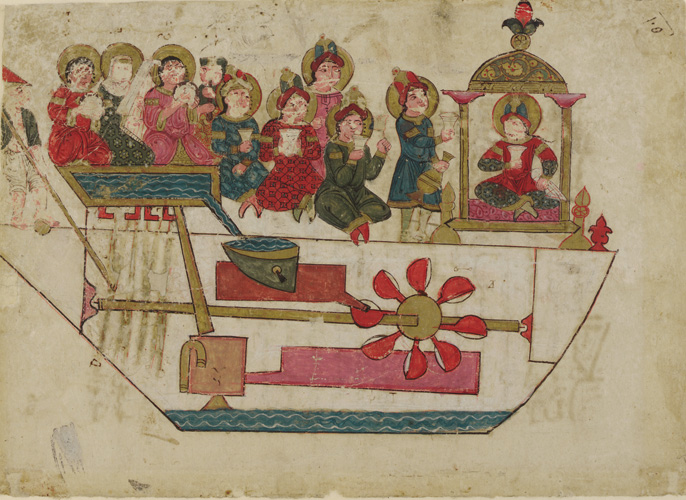
\includegraphics[width=1\linewidth]{chapters/chapter1/images/1}
		\caption{Музыкальная лодка Аль-Джазири.}
		\label{ris:image1x1}
	\end{center}
\end{figure}

Не обошел вниманием создание робота и другой известнейший изобретатель средневековья~--- Леонардо да Винчи. Среди его бумаг найдены разработки человекоподобного робота, одетого в германо-итальянскую броню. Робот был запрограммирован имитировать человеческие движения (приподниматься и садиться, двигать руками и шеей), и имел анатомически правильное строение челюсти. Технология частично основывалась на исследованиях Леонардо в анатомии, в частности Витрувианском человеке. Неизвестно был ли этот проект воплощен в реальность.
\clearpage
\begin{figure}[h!]
	\begin{center}
		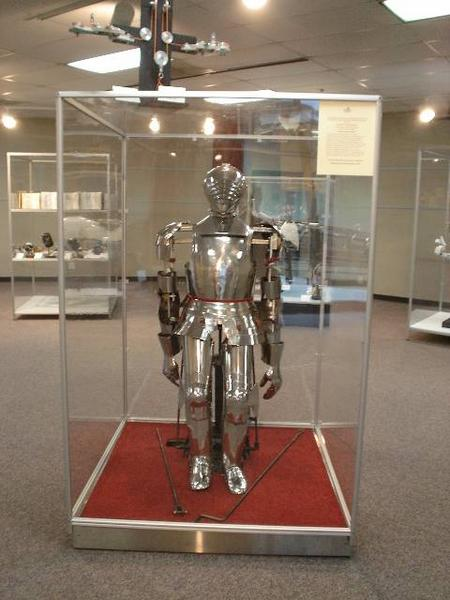
\includegraphics[width=1\linewidth]{chapters/chapter1/images/2}
		\caption{Реконструкция робота Леонардо, выполненная Марио Таддеи.}
		\label{ris:image1x2}
	\end{center}
\end{figure}

Затем были многочисленные автоматические инструменты, танцоры, звери. Выполненные в основном из дерева они могли выполнять десятки различных действий по заложенной программе. Разумеется, ни о какой полезной нагрузке речи не шло, это были  роскошные механизмы, служившие для увеселения богатых граждан.

Век за веком, повторяя общую историю развития техники, появлялись роботы на паровой тяге,  первые электрические роботы, наконец, роботы на полупроводниковой электронике.

{\slshape Если во вступление не включены интерактивные моменты, затягивать его не стоит. После краткого обзора учащимся предлагается следующая викторина.}\\\\

{\hypertarget{lesson1x3}{\blackBlueText{III. Роботы из кинофильмов.}}}\\\\

Викторину можно проводить как для команд, так и для всех учащихся индивидуально. На проекторе демонстрируются кадры из знаменитых фильмов про роботов. По поднятой руке команда (учащийся) получает право ответить на вопрос «Как зовут этого робота и в каком фильме (фильмах) его можно увидеть?». Правильный и полный ответ приносит команде очко, в противном случае право ответа получает следующая по очередности команда.

После того, как робот угадан, рекомендуется показать подготовленные отрывки из кинофильма, на которых хорошо видны конструкционные особенности, возможности и способы передвижения робота и обсудить их с учащимися. 

{\slshape Рекомендации по подобным отрывкам можно найти в Приложении. Ниже представлены возможные варианты вопросов.}
\begin{figure}[h!]
	\begin{center}
		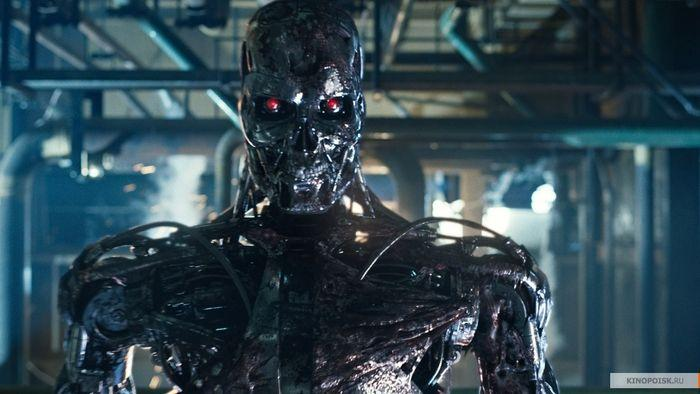
\includegraphics[width=0.98\linewidth]{chapters/chapter1/images/3}
		\caption{Терминатор. Фильмы «Терминатор» 1-5.}
		\label{ris:image1x3}
	\end{center}
\end{figure}
\begin{figure}[h!]
	\begin{center}
		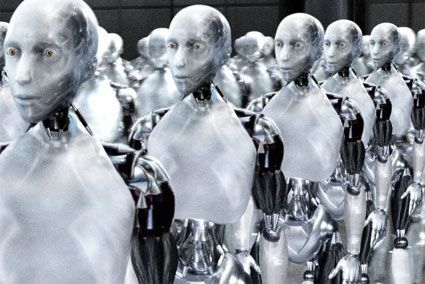
\includegraphics[width=0.98\linewidth]{chapters/chapter1/images/4}
		\caption{Робот Санни. Фильм «Я, робот».}
		\label{ris:image1x4}
	\end{center}
\end{figure}
\begin{figure}[h!]
	\begin{center}
		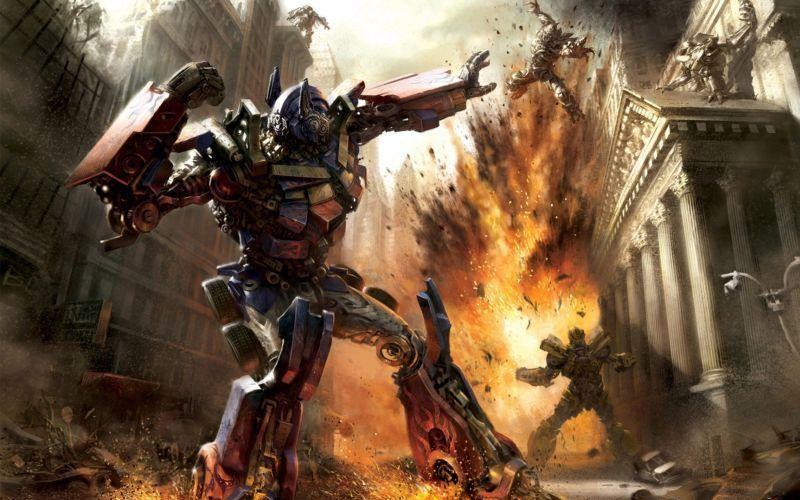
\includegraphics[width=0.98\linewidth]{chapters/chapter1/images/5}
		\caption{Робот Оптимус Прайм. Фильм «Трансформеры» 1,2.}
		\label{ris:image1x5}
	\end{center}
\end{figure}
\begin{figure}[h!]
	\begin{center}
		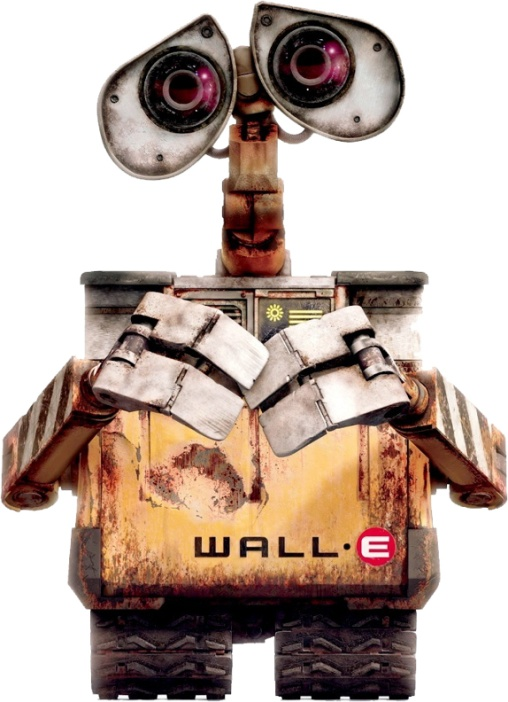
\includegraphics[width=1\linewidth]{chapters/chapter1/images/6}
		\caption{Робот Валли из одноименного фильма.}
		\label{ris:image1x6}
	\end{center}
\end{figure}	
\begin{figure}[h!]
	\begin{center}
		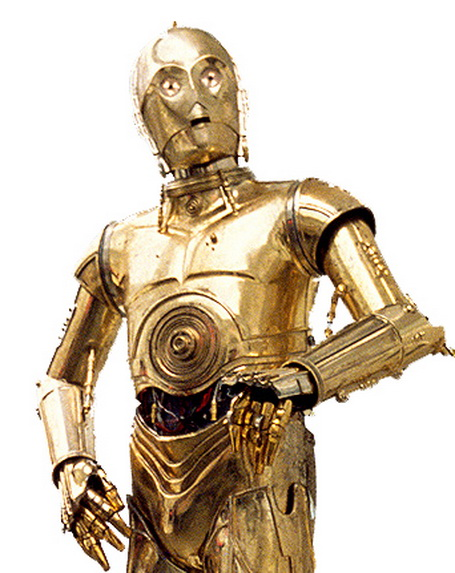
\includegraphics[width=1\linewidth]{chapters/chapter1/images/7}
		\caption{Робот С3РО. Фильм «Звездные войны», 1-6.}
		\label{ris:image1x7}
	\end{center}
\end{figure}
\begin{figure}[h!]
	\begin{center}
		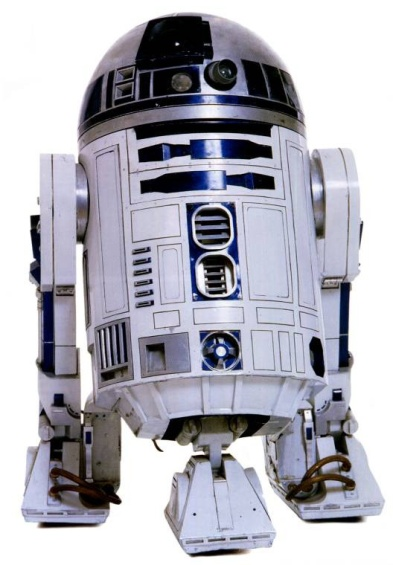
\includegraphics[width=1\linewidth]{chapters/chapter1/images/8}
		\caption{Робот R2D2. Фильм «Звездные войны», 1-6.}
		\label{ris:image1x8}
	\end{center}
\end{figure}
\clearpage
\begin{figure}[h!]
	\begin{center}
		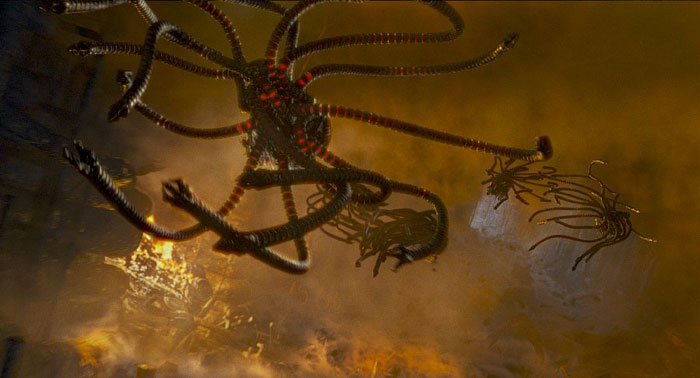
\includegraphics[width=1\linewidth]{chapters/chapter1/images/9}
		\caption{Безымянные роботы-охотники. Фильм «Матрица» 1-3.}
		\label{ris:image1x9}
	\end{center}
\end{figure}	

{\hypertarget{lesson1x4}{\blackBlueText{IV. Классификация роботов.}}}\\\\

Миры ближайшего будущего в кино полны роботов, кажется рукой подать до  эры «настоящих» роботов, роботов-помощников, выполняющих за человека всю тяжелую и нудную работу. Ожидание, правда тянется уже лет 40. Когда же уже роботы будут среди нас? А может быть они уже \dots?

Небезызвестный робот~--- пылесос~--- не робот? А точнейший механический манипулятор, собирающий  машины на заводе~--- не робот? А холодильник, заказывающий недостающие продукты в Интернете? Уже нет?  А  марсоход  Curiosity? Да? А смартфон в вашем кармане? Нет?  Так кто же такой, этот загадочный робот?

На самом деле грани тут, конечно, очень тонкие и условные. И необходимость в классификации роботов и выделении различных направлений робототехники назрела очень серьезная, робототехника еще ждет своего Линнея. В рамках нашего курса мы ограничимся вот такой простейшей классификацией:
\clearpage
\begin{figure}[h!]
	\begin{center}
		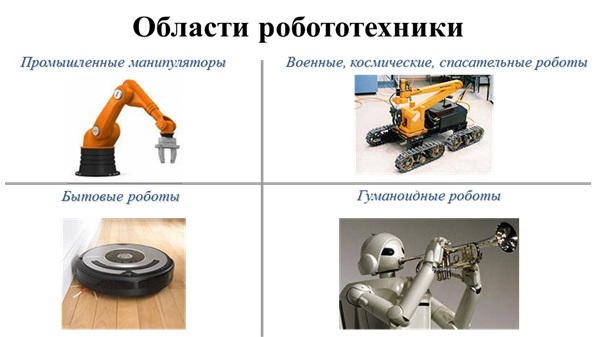
\includegraphics[width=1\linewidth]{chapters/chapter1/images/10}
		\caption{Области современной робототехники.}
		\label{ris:image1x10}
	\end{center}
\end{figure}		

В рамках нашего курса мы коснемся всех направлений. Вы создадите и управляемые, и автономные конструкции. Смоделируете, если не всего человека, то хотя бы его часть. Соберете сложный манипулятор с простым управлением и простую тележку, со сложным поведением. И. конечно, решите самую сложную задачу~--- творческую, создав своего уникального робота. Он будет заваривать чай и приносить тапочки? Имитировать полет мотылька к свету? Или включать дома отопление по SMS-команде? Скоро узнаем!\\\\

{\hypertarget{lesson1x5}{\blackBlueText{V. «Фантазийный робот»}}}\\\\

В заключение первого занятия предлагается провести творческое соревнование по созданию проекта собственного робота. Учащимся предлагается придумать и описать концепцию робота, которого они хотели бы создать. Приветствуются любые рисунки, модели. По желанию допустима как работа в командах, так и индивидуальное творчество.

Дайте толчок к творчеству, предложите детям использовать карандаши, клей, цветной картон, пластилин, пластиковые бутылки, скотч, трубочки для коктейлей, деревянные палочки для шашлыков, канцелярские резинки, пакеты.

На сам процесс творчества отводится примерно 30 минут. В конце проводится краткое представление учащимися своего робота. Вопросы для обсуждения:

\begin{enumerate}
	\item Что делает этот робот?
	\item Как он выполняет свою работу, какие конструкционные особенности ему в этом помогают?
	\item Кому пригодится такой робот?
\end{enumerate}
Можно так же провести голосование и выбрать лучших роботов в следующих номинациях:

\begin{enumerate}
	\item Самый лучший дизайн робота.
	\item Самая продуманная концепция.
	\item Самый нужный человечеству робот.	
\end{enumerate}
{\slshape Материалы, созданные учащимися, сохраните, они еще несколько раз понадобятся в течение курса.}